%% bare_jrnl.tex
%% V1.4b
%% 2015/08/26
%% by Michael Shell
%% see http://www.michaelshell.org/
%% for current contact information.
%%
%% This is a skeleton file demonstrating the use of IEEEtran.cls
%% (requires IEEEtran.cls version 1.8b or later) with an IEEE
%% journal paper.
%%
%% Support sites:
%% http://www.michaelshell.org/tex/ieeetran/
%% http://www.ctan.org/pkg/ieeetran
%% and
%% http://www.ieee.org/

%%*************************************************************************
%% Legal Notice:
%% This code is offered as-is without any warranty either expressed or
%% implied; without even the implied warranty of MERCHANTABILITY or
%% FITNESS FOR A PARTICULAR PURPOSE! 
%% User assumes all risk.
%% In no event shall the IEEE or any contributor to this code be liable for
%% any damages or losses, including, but not limited to, incidental,
%% consequential, or any other damages, resulting from the use or misuse
%% of any information contained here.
%%
%% All comments are the opinions of their respective authors and are not
%% necessarily endorsed by the IEEE.
%%
%% This work is distributed under the LaTeX Project Public License (LPPL)
%% ( http://www.latex-project.org/ ) version 1.3, and may be freely used,
%% distributed and modified. A copy of the LPPL, version 1.3, is included
%% in the base LaTeX documentation of all distributions of LaTeX released
%% 2003/12/01 or later.
%% Retain all contribution notices and credits.
%% ** Modified files should be clearly indicated as such, including  **
%% ** renaming them and changing author support contact information. **
%%*************************************************************************


% *** Authors should verify (and, if needed, correct) their LaTeX system  ***
% *** with the testflow diagnostic prior to trusting their LaTeX platform ***
% *** with production work. The IEEE's font choices and paper sizes can   ***
% *** trigger bugs that do not appear when using other class files.       ***                          ***
% The testflow support page is at:
% http://www.michaelshell.org/tex/testflow/



\documentclass[journal]{IEEEtran}
\usepackage[brazilian]{babel}
\usepackage[utf8]{inputenc}
\usepackage[T1]{fontenc}
%
% If IEEEtran.cls has not been installed into the LaTeX system files,
% manually specify the path to it like:
% \documentclass[journal]{../sty/IEEEtran}





% Some very useful LaTeX packages include:
% (uncomment the ones you want to load)


% *** MISC UTILITY PACKAGES ***
%
%\usepackage{ifpdf}
% Heiko Oberdiek's ifpdf.sty is very useful if you need conditional
% compilation based on whether the output is pdf or dvi.
% usage:
% \ifpdf
%   % pdf code
% \else
%   % dvi code
% \fi
% The latest version of ifpdf.sty can be obtained from:
% http://www.ctan.org/pkg/ifpdf
% Also, note that IEEEtran.cls V1.7 and later provides a builtin
% \ifCLASSINFOpdf conditional that works the same way.
% When switching from latex to pdflatex and vice-versa, the compiler may
% have to be run twice to clear warning/error messages.






% *** CITATION PACKAGES ***
%
%\usepackage{cite}
% cite.sty was written by Donald Arseneau
% V1.6 and later of IEEEtran pre-defines the format of the cite.sty package
% \cite{} output to follow that of the IEEE. Loading the cite package will
% result in citation numbers being automatically sorted and properly
% "compressed/ranged". e.g., [1], [9], [2], [7], [5], [6] without using
% cite.sty will become [1], [2], [5]--[7], [9] using cite.sty. cite.sty's
% \cite will automatically add leading space, if needed. Use cite.sty's
% noadjust option (cite.sty V3.8 and later) if you want to turn this off
% such as if a citation ever needs to be enclosed in parenthesis.
% cite.sty is already installed on most LaTeX systems. Be sure and use
% version 5.0 (2009-03-20) and later if using hyperref.sty.
% The latest version can be obtained at:
% http://www.ctan.org/pkg/cite
% The documentation is contained in the cite.sty file itself.






% *** GRAPHICS RELATED PACKAGES ***
%
\ifCLASSINFOpdf
  \usepackage[pdftex]{graphicx}
  % declare the path(s) where your graphic files are
  \graphicspath{{./img/}}
  % and their extensions so you won't have to specify these with
  % every instance of \includegraphics
  \DeclareGraphicsExtensions{.pdf,.jpeg,.png}
\else
  % or other class option (dvipsone, dvipdf, if not using dvips). graphicx
  % will default to the driver specified in the system graphics.cfg if no
  % driver is specified.
  % \usepackage[dvips]{graphicx}
  % declare the path(s) where your graphic files are
  % \graphicspath{{../eps/}}
  % and their extensions so you won't have to specify these with
  % every instance of \includegraphics
  % \DeclareGraphicsExtensions{.eps}
\fi
% graphicx was written by David Carlisle and Sebastian Rahtz. It is
% required if you want graphics, photos, etc. graphicx.sty is already
% installed on most LaTeX systems. The latest version and documentation
% can be obtained at: 
% http://www.ctan.org/pkg/graphicx
% Another good source of documentation is "Using Imported Graphics in
% LaTeX2e" by Keith Reckdahl which can be found at:
% http://www.ctan.org/pkg/epslatex
%
% latex, and pdflatex in dvi mode, support graphics in encapsulated
% postscript (.eps) format. pdflatex in pdf mode supports graphics
% in .pdf, .jpeg, .png and .mps (metapost) formats. Users should ensure
% that all non-photo figures use a vector format (.eps, .pdf, .mps) and
% not a bitmapped formats (.jpeg, .png). The IEEE frowns on bitmapped formats
% which can result in "jaggedy"/blurry rendering of lines and letters as
% well as large increases in file sizes.
%
% You can find documentation about the pdfTeX application at:
% http://www.tug.org/applications/pdftex





% *** MATH PACKAGES ***
%
%\usepackage{amsmath}
% A popular package from the American Mathematical Society that provides
% many useful and powerful commands for dealing with mathematics.
%
% Note that the amsmath package sets \interdisplaylinepenalty to 10000
% thus preventing page breaks from occurring within multiline equations. Use:
%\interdisplaylinepenalty=2500
% after loading amsmath to restore such page breaks as IEEEtran.cls normally
% does. amsmath.sty is already installed on most LaTeX systems. The latest
% version and documentation can be obtained at:
% http://www.ctan.org/pkg/amsmath





% *** SPECIALIZED LIST PACKAGES ***
%
%\usepackage{algorithmic}
% algorithmic.sty was written by Peter Williams and Rogerio Brito.
% This package provides an algorithmic environment fo describing algorithms.
% You can use the algorithmic environment in-text or within a figure
% environment to provide for a floating algorithm. Do NOT use the algorithm
% floating environment provided by algorithm.sty (by the same authors) or
% algorithm2e.sty (by Christophe Fiorio) as the IEEE does not use dedicated
% algorithm float types and packages that provide these will not provide
% correct IEEE style captions. The latest version and documentation of
% algorithmic.sty can be obtained at:
% http://www.ctan.org/pkg/algorithms
% Also of interest may be the (relatively newer and more customizable)
% algorithmicx.sty package by Szasz Janos:
% http://www.ctan.org/pkg/algorithmicx




% *** ALIGNMENT PACKAGES ***
%
%\usepackage{array}
% Frank Mittelbach's and David Carlisle's array.sty patches and improves
% the standard LaTeX2e array and tabular environments to provide better
% appearance and additional user controls. As the default LaTeX2e table
% generation code is lacking to the point of almost being broken with
% respect to the quality of the end results, all users are strongly
% advised to use an enhanced (at the very least that provided by array.sty)
% set of table tools. array.sty is already installed on most systems. The
% latest version and documentation can be obtained at:
% http://www.ctan.org/pkg/array


% IEEEtran contains the IEEEeqnarray family of commands that can be used to
% generate multiline equations as well as matrices, tables, etc., of high
% quality.




% *** SUBFIGURE PACKAGES ***
%\ifCLASSOPTIONcompsoc
%  \usepackage[caption=false,font=normalsize,labelfont=sf,textfont=sf]{subfig}
%\else
%  \usepackage[caption=false,font=footnotesize]{subfig}
%\fi
% subfig.sty, written by Steven Douglas Cochran, is the modern replacement
% for subfigure.sty, the latter of which is no longer maintained and is
% incompatible with some LaTeX packages including fixltx2e. However,
% subfig.sty requires and automatically loads Axel Sommerfeldt's caption.sty
% which will override IEEEtran.cls' handling of captions and this will result
% in non-IEEE style figure/table captions. To prevent this problem, be sure
% and invoke subfig.sty's "caption=false" package option ([Online] Disponível since
% subfig.sty version 1.3, 2005/06/28) as this is will preserve IEEEtran.cls
% handling of captions.
% Note that the Computer Society format requires a larger sans serif font
% than the serif footnote size font used in traditional IEEE formatting
% and thus the need to invoke different subfig.sty package options depending
% on whether compsoc mode has been enabled.
%
% The latest version and documentation of subfig.sty can be obtained at:
% http://www.ctan.org/pkg/subfig




% *** FLOAT PACKAGES ***
%
%\usepackage{fixltx2e}
% fixltx2e, the successor to the earlier fix2col.sty, was written by
% Frank Mittelbach and David Carlisle. This package corrects a few problems
% in the LaTeX2e kernel, the most notable of which is that in current
% LaTeX2e releases, the ordering of single and double column floats is not
% guaranteed to be preserved. Thus, an unpatched LaTeX2e can allow a
% single column figure to be placed prior to an earlier double column
% figure.
% Be aware that LaTeX2e kernels dated 2015 and later have fixltx2e.sty's
% corrections already built into the system in which case a warning will
% be issued if an attempt is made to load fixltx2e.sty as it is no longer
% needed.
% The latest version and documentation can be found at:
% http://www.ctan.org/pkg/fixltx2e


%\usepackage{stfloats}
% stfloats.sty was written by Sigitas Tolusis. This package gives LaTeX2e
% the ability to do double column floats at the bottom of the page as well
% as the top. (e.g., "\begin{figure*}[!b]" is not normally possible in
% LaTeX2e). It also provides a command:
%\fnbelowfloat
% to enable the placement of footnotes below bottom floats (the standard
% LaTeX2e kernel puts them above bottom floats). This is an invasive package
% which rewrites many portions of the LaTeX2e float routines. It may not work
% with other packages that modify the LaTeX2e float routines. The latest
% version and documentation can be obtained at:
% http://www.ctan.org/pkg/stfloats
% Do not use the stfloats baselinefloat ability as the IEEE does not allow
% \baselineskip to stretch. Authors submitting work to the IEEE should note
% that the IEEE rarely uses double column equations and that authors should try
% to avoid such use. Do not be tempted to use the cuted.sty or midfloat.sty
% packages (also by Sigitas Tolusis) as the IEEE does not format its papers in
% such ways.
% Do not attempt to use stfloats with fixltx2e as they are incompatible.
% Instead, use Morten Hogholm'a dblfloatfix which combines the features
% of both fixltx2e and stfloats:
%
% \usepackage{dblfloatfix}
% The latest version can be found at:
% http://www.ctan.org/pkg/dblfloatfix




%\ifCLASSOPTIONcaptionsoff
%  \usepackage[nomarkers]{endfloat}
% \let\MYoriglatexcaption\caption
% \renewcommand{\caption}[2][\relax]{\MYoriglatexcaption[#2]{#2}}
%\fi
% endfloat.sty was written by James Darrell McCauley, Jeff Goldberg and 
% Axel Sommerfeldt. This package may be useful when used in conjunction with 
% IEEEtran.cls'  captionsoff option. Some IEEE journals/societies require that
% submissions have lists of figures/tables at the end of the paper and that
% figures/tables without any captions are placed on a page by themselves at
% the end of the document. If needed, the draftcls IEEEtran class option or
% \CLASSINPUTbaselinestretch interface can be used to increase the line
% spacing as well. Be sure and use the nomarkers option of endfloat to
% prevent endfloat from "marking" where the figures would have been placed
% in the text. The two hack lines of code above are a slight modification of
% that suggested by in the endfloat docs (section 8.4.1) to ensure that
% the full captions always appear in the list of figures/tables - even if
% the user used the short optional argument of \caption[]{}.
% IEEE papers do not typically make use of \caption[]'s optional argument,
% so this should not be an issue. A similar trick can be used to disable
% captions of packages such as subfig.sty that lack options to turn off
% the subcaptions:
% For subfig.sty:
% \let\MYorigsubfloat\subfloat
% \renewcommand{\subfloat}[2][\relax]{\MYorigsubfloat[]{#2}}
% However, the above trick will not work if both optional arguments of
% the \subfloat command are used. Furthermore, there needs to be a
% description of each subfigure *somewhere* and endfloat does not add
% subfigure captions to its list of figures. Thus, the best approach is to
% avoid the use of subfigure captions (many IEEE journals avoid them anyway)
% and instead reference/explain all the subfigures within the main caption.
% The latest version of endfloat.sty and its documentation can obtained at:
% http://www.ctan.org/pkg/endfloat
%
% The IEEEtran \ifCLASSOPTIONcaptionsoff conditional can also be used
% later in the document, say, to conditionally put the References on a 
% page by themselves.




% *** PDF, URL AND HYPERLINK PACKAGES ***
%
%\usepackage{url}
% url.sty was written by Donald Arseneau. It provides better support for
% handling and breaking URLs. url.sty is already installed on most LaTeX
% systems. The latest version and documentation can be obtained at:
% http://www.ctan.org/pkg/url
% Basically, \url{my_url_here}.




% *** Do not adjust lengths that control margins, column widths, etc. ***
% *** Do not use packages that alter fonts (such as pslatex).         ***
% There should be no need to do such things with IEEEtran.cls V1.6 and later.
% (Unless specifically asked to do so by the journal or conference you plan
% to submit to, of course. )


% correct bad hyphenation here
\hyphenation{op-tical net-works semi-conduc-tor}


\begin{document}
%
% paper title
% Titles are generally capitalized except for words such as a, an, and, as,
% at, but, by, for, in, nor, of, on, or, the, to and up, which are usually
% not capitalized unless they are the first or last word of the title.
% Linebreaks \\ can be used within to get better formatting as desired.
% Do not put math or special symbols in the title.
\title{IoT - A Internet das coisas}
%
%
% author names and IEEE memberships
% note positions of commas and nonbreaking spaces ( ~ ) LaTeX will not break
% a structure at a ~ so this keeps an author's name from being broken across
% two lines.
% use \thanks{} to gain access to the first footnote area
% a separate \thanks must be used for each paragraph as LaTeX2e's \thanks
% was not built to handle multiple paragraphs
%

\author{Willian Marques Freire e
        Munif Gebara Junior% <-this % stops a space
\thanks{Faculdade de Filosofia Ciências e Letras de Mandaguari é uma fundação
situada em Mandaguari no Paraná região sul brasileira,
na rua Rene Taccola, 152 - Centro Site: (see http://www.fafiman.br/index.html).}% <-this % stops a space
\thanks{Artigo realizado em 2017.}}

% note the % following the last \IEEEmembership and also \thanks - 
% these prevent an unwanted space from occurring between the last author name
% and the end of the author line. i.e., if you had this:
% 
% \author{....lastname \thanks{...} \thanks{...} }
%                     ^------------^------------^----Do not want these spaces!
%
% a space would be appended to the last name and could cause every name on that
% line to be shifted left slightly. This is one of those "LaTeX things". For
% instance, "\textbf{A} \textbf{B}" will typeset as "A B" not "AB". To get
% "AB" then you have to do: "\textbf{A}\textbf{B}"
% \thanks is no different in this regard, so shield the last } of each \thanks
% that ends a line with a % and do not let a space in before the next \thanks.
% Spaces after \IEEEmembership other than the last one are OK (and needed) as
% you are supposed to have spaces between the names. For what it is worth,
% this is a minor point as most people would not even notice if the said evil
% space somehow managed to creep in.



% The paper headers
\markboth{IoT - A Internet das Coisas,~Vol.~1, No.~1, Julho~2017}%
{Shell \MakeLowercase{\textit{et al.}}: Bare Demo of IEEEtran.cls for IEEE Journals}
% The only time the second header will appear is for the odd numbered pages
% after the title page when using the twoside option.
% 
% *** Note that you probably will NOT want to include the author's ***
% *** name in the headers of peer review papers.                   ***
% You can use \ifCLASSOPTIONpeerreview for conditional compilation here if
% you desire.




% If you want to put a publisher's ID mark on the page you can do it like
% this:
%\IEEEpubid{0000--0000/00\$00.00~\copyright~2015 IEEE}
% Remember, if you use this you must call \IEEEpubidadjcol in the second
% column for its text to clear the IEEEpubid mark.



% use for special paper notices
%\IEEEspecialpapernotice{(Invited Paper)}




% make the title area
\maketitle

% As a general rule, do not put math, special symbols or citations
% in the abstract or keywords.
\begin{abstract}
The abstract goes here.
\end{abstract}

% Note that keywords are not normally used for peerreview papers.
\begin{IEEEkeywords}
IEEE, IEEEtran, journal, \LaTeX, paper, template.
\end{IEEEkeywords}






% For peer review papers, you can put extra information on the cover
% page as needed:
% \ifCLASSOPTIONpeerreview
% \begin{center} \bfseries EDICS Category: 3-BBND \end{center}
% \fi
%
% For peerreview papers, this IEEEtran command inserts a page break and
% creates the second title. It will be ignored for other modes.
\IEEEpeerreviewmaketitle



\section{Introdução}
% The very first letter is a 2 line initial drop letter followed
% by the rest of the first word in caps.
% 
% form to use if the first word consists of a single letter:
% \IEEEPARstart{A}{demo} file is ....
% 
% form to use if you need the single drop letter followed by
% normal text (unknown if ever used by the IEEE):
% \IEEEPARstart{A}{}demo file is ....
% 
% Some journals put the first two words in caps:
% \IEEEPARstart{T}{his demo} file is ....
% 
% Here we have the typical use of a "T" for an initial drop letter
% and "HIS" in caps to complete the first word.
\IEEEPARstart{I}{ot} ou Internet das coisas, algumas vezes referida como a Internet dos objetos, está gerando uma revolução tecnológica em diversas áreas e inclusive na humanidade. Considerando que o IoT representa a próxima evolução da Internet, dando um salto na capacidade de coletar, analisar e distribuir dados, faz-se com que os mesmos possam ser transformados em informação. Atualmente existem projetos IoT em desenvolvimento, que prometem fechar a lacuna entre ricos e pobres, melhorando a distribuição dos recursos mundiais para aqueles que precisam deles, e ajudando a entender a sociedade atual para que possa ser mais proativa e menos reativa \cite[p.~2]{Evans}.

Segundo o Artigo Internet of Things volume III, na empresa Dzone (empresa que faz publicações online sobre tecnologia) encontram-se 797 profissionais que são responsáveis pela área de IoT, e uma das maiores preocupações da mesma é este âmbito. Em um inquérito realizado pela mesma, foi perguntado sobre as maiores preocupações quando se trata de IoT. O centro de preocupação estava pela segurança e privacidade, pois os mesmos, estavam interessados em IoT para o contexto empresarial de suas empresas. A falta de padrões, era um terço na coluna ''muito preocupada'' chegando a 34\% dos envolvidos. Dentre eles, 25\% dos entrevistados desconfiam da conectividade e do baixo custo de energia, sendo que 24\% se preocupam com a manutenção de hardware e software, e 14\% estão apreensivos com o desenvolvimento imaturo e paradigmas de redes \cite[p.~4]{Evans}.

Em 1999 foi fundado um grupo chamado MIT (Massachusetts Institute of Technology), que tem trabalhado no campo de identificação de frequência de rádio, em rede (RFID) e tecnologias de sensores emergentes. Em 2003, haviam aproximadamente 6,3 bilhões de pessoas vivendo no mundo, e aproximadamente 500 milhões de dispositivos conectados à internet. O crescimento mastodôntico de smartphones e tablets, elevou o número de dispositivos conectados a Internet para aproximadamente 12,5 bilhões em 2010 \cite[p.~3]{Evans}.

Em janeiro de 2009, uma equipe de pesquisadores chinesa, finalizou um estudo sobre os dados de roteamento da internet em intervalos de seis meses, entre dezembro de 2001 e dezembro de 2006. Foi descoberto pelos mesmos, que a Internet dobra de tamanho a cada 5,32 anos (EVERS, 2003). Em um dos artigos publicados por Evans \cite{Evans}, o mesmo faz a citação de um gráfico feito pelo Cisco ISBG - multinacional estadunidense sediada em San José na Califórnia, que refina esta pesquisa. 

\begin{figure}[h]
\centering
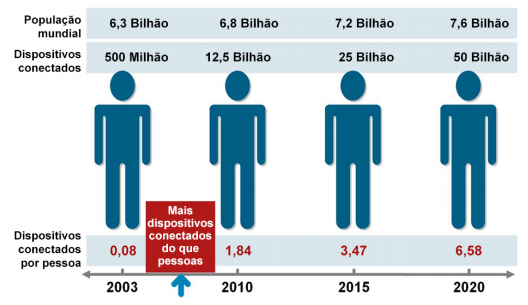
\includegraphics[width=2.5in]{um}
\caption{"Nascimento" do IoT entre 2008 e 2009 \cite{Evans}.}
\label{fig_um}
\end{figure}


A Internet têm transcorrido por diversas etapas evolucionárias distintas. A primeira fase existente foi quando a Web foi chamada de ARPANET (Advanced Research Projects Agency Network). A segunda fase da Web foi caracterizada pela concentração de todas as empresas, compartilharem informações na Internet para divulgação de produtos e serviços. Seguido por uma terceira evolução, que mudou a Web de um estágio com informações estáticas para informações transacionais, nas quais produtos e serviços são comercializados totalmente online. Após todas estas evoluções, surge a quarta etapa, onde é criado o conceito de Web social e experiência do usuário, na qual empresas como Facebook, Twitter se tornaram famosas e profícuas, ao permitir que pessoas se comuniquem e compartilhem informações \cite[p.~6]{Evans}.

IoT Tem mudado o modelo de hardware computacional, que nasceu a aproximadamente 40 anos atrás. Considerando todas as fases diferentes de modelos de hardware que existiram, dentre elas micro-computadores pessoais, e hoje computadores conectados na nuvem expandindo o modelo cliente-servidor para novos paradigmas, comprova que a cada revolução IoT surge a necessidade de modificar este modelo \cite[p.~6]{dzonevoltreeiot}. Devido a diversos estudos visando melhor desenvolvimento e aproveitamento do modelo cliente-servidor, surgiram vários protocolos para transmissão de dados. O protocolo principal utilizado atualmente é o HTTP (Hypertext Transfer Protocol) encontrando-se por padrão em praticamente quase todos os navegadores atuais, existem ainda outros protocolos como FTP (File Transfer Protocol) para transferência de arquivos, IMAP (IInternet Message Access Protocol) para envio de Mensagens, entre outros. 

Aproveitando-se destes protocolos, também surgiu especificações e arquiteturas, para que aplicações possam se disponibilizadas como serviços, dentre elas encontra-se o REST (Representational State Transfer) ou Transferência de Estado representacional, que segundo Fielding \cite{roythomasfielding2017}, é uma abstração da arquitetura World Wide Web, um estilo  arquitetural, que consiste em um conjunto coordenado de restições arquiteturais aplicadas a componentes, conectores e elementos de dados dentro de um sistema de hipermídia distribuído, entretanto, é um assunto para o próximo artigo que será falado sobre Micro-serviços.

O objetivo deste trabalho, é exemplificar o processo de criação de uma estrutura IoT, e demonstrar duas lacunas. A primeira é a configuração de um dispositivo IoT de forma simples, que será preenchida durante este trabalho, e a outra, é preechida no artigo Micro-serviços de Marques e Gebara \cite{MarquesMunif}, ao ser estudado sobre a integração de IoT e micro-serviços, que diz sobre quando é necessário ser compartilhado estas informações dos dispositivos, não somente em rede interna, mas externa. O que será construído durante este trabalho, é uma estrutura IoT flexível, que seja capaz de se comunicar através do protocolo HTTP com serviços WEB, que ficarão encarregados de compartilhar as informações recebidas dos dispositivos IoT pela Internet.

% You must have at least 2 lines in the paragraph with the drop letter
% (should never be an issue)
I wish you the best of success.

\hfill mds
 
\hfill 13 de Maio de 2017

\subsection{Revisão Bibliográfica}
\subsubsection{IoT}

Atualmente, existem diversos tipos e marcas de placas com circuito integrado e computadores, para desenvolvimento IoT. Em uma nova pesquisa realizada pelo Dzone, foram entrevistadors diversas pessoas, para obter um percentual de preferência entre os dispositivos. Dentre os mesmos, 53\% preferem Rapberry Pi, 28\% preferem o Arduino, e 19\% não apresentam nenhuma preferência. Nesta pesquisa, foram relatados protocolos mais utilizados dentro do ramo IoT. Dentre os entrevistados, 14\% disseram ter preferência por Wifi-Direct em produção, 8\% preferem utilizar Bluetooh LE em ambientes que não são de produção. No total, 24\% já havia utilizado Wifi-Direct e 23\% Bluetookh LE. Um protocolo também citado, é o MQTT (Message Queue Telemetry Transport), que segundo o site FilipeFlop \cite{filipeflopnodemcu}, é um protocolo de mensagens leve, criado para comunicação M2M (Machine to Machine),  obteve 33\% de preferência de utilização em produção \cite[p.~4]{dzoneiotvolume4}.

Assim como aplicações web ou móveis, dispositivos físicos também precisam ser consensuais. No entanto, existem desafios adicionais para o IoT. As arquiteturas atuais ainda deixam a desejar em questão de terminais e configuração. Uma segunda preocupação na área de IoT é o tempo necessário para atualização de software para o dispositivo. Dentre as  complicações que poder existir, a vulnerabilidade de um dispositivo, pode ser alvo para ataques e invasões. Uma das maneiras de gerenciar a testabilidade do software no dispositivo, é testar isoladamente. Reproduzir o ecossistema em torno do dispositivo e como os usuários interagem garantem uma boa testabilidade. Além destes aspectos, complexos sistemas sociotécnicos cercam a humanidade. Estudos avançados reconhecem que não se podem identificar, e muito menos testar cada possível cenário de falha. Por este fato, estes estudos concentram cada vez mais na confiabilidade. O ultimo desafio para área de IoT, são as identificações e dignosticação de falhas. Tomar ações rapidamente para resolução de problemas, é um aspecto fundamental no desenvolvimento de dispositivos IoT. Técnicas para integração continua são utilizados para resolver estes problemas, uma delas é a Canary Release, que Segundo Danilo Sato \cite{danilosato2017}, é uma técnica para reduzir o risco de introduzir uma nova versão de software na produção, lançando mudanças lentamente para um pequeno subconjunto de usuários, antes de lança-la em toda a infra-estrutura e torná-la disponível para todos \cite[p.~9]{dzoneiotvolume4}.

Nas últimas duas décadas, houveram avanços tecnológicos na área computacional, surgindo processadores com mais capacidade de processamento, armazenamentos, memória e dispositivos de rede com baixo custo. Atualmente, dispositivos físicos estão sendo desenvolvidos com mais capacidade compitacional, e interligados atrabés da internet de maneira efetiva. A adoção generalizada das tecnologias IoT enriquecem a idéia de computação ubíqua, um conceito que surgiu no final dos anos 80. Segundo Mark Weiser,  criador do conceito citado, escreveu em seu artigo The Computer for the 21st Century, que o computador se integra a vida das pessoas de modo que elas não o percebam, entretanto, o utilizem. Motivado por esta convicção, Weiser percebeu que em sua época não haviam tecnologias necessárias para que a Computação Ubíqua se tornasse realidade, fazendo com que assim, dedicasse esforços para desenvolver estes meios.  \cite{MarkWeiser}.

Em um artigo feito pelo professor Michael Wooldridge, chefe do Departamento de Ciência da Computação da Universidade de Oxford, o mesmo definiu um termo utilizado no meio tecnológico, que são os agentes. Sendo ele, um agente é: um computador que está situado em algum ambiente, capaz de realizar ações autônomas sobre este, para cumprir seus objetivos delegados. O mesmo torna-se inteligente com as seguintes propriedades: Reatividade (a percepção de seu ambiente, e a capacidade de respota em tempo hábil sobre mudanças que ocorrem), proatividade (antecipação de problemas futuros), habilidade social (capacidade de interação entre agentes para satisfazer seus objetivos de design) \cite{MichaelWooldridge}.

No início de 1926, uma revista chamada Collier publicou uma entrevista com Nikola Tesla, no qual ele falou sobre suas previsões para as próximas décadas. Entre elas, ele falava de um mundo com máquinas voadoras, energia sem fio e superioridade feminina. Segundo palavras de Tesla. quando a tecnologia sem fio estivesse perfeitamente estabelecida em todo o mundo, o planeta se tornaria um enorme cérebro. Nesta entrvista, ele disse qua inclusive os ser humano seria capaz de se comunicar uns com os outros de imediato, independente da distância \cite{johnBKennedy}.

\subsubsection{NodeMCU}

Neste trabalho, será utilizado o NodeMCU para desenvolvimento das aplicaçoes IoT, pelo fato do mesmo conter um módulo WiFi, o que facilitará na comunicação via interface de rede com os micro-serviços. NodeMCU é um firmware baseado em eLua - uma implementação completa utilizando programação Lua para sistemas embarcados \cite{elua2017}. O mesmo foi projetado para ser integrado com o Chip WiFi ESP8266 desenvolvido pela empresa Espressif, situada em Shangai, especializada no ramo de IoT \cite{systems}. O NodeMCU utiliza sistema de arquivos SPIFFS (SPI Flash File System) e seu repositório no Github consiste em 98.1\% de código na linguagem C - criada em 1972 por Dennis Ritchie \cite{williamstewart2017} e o demais existente em código escrito na linguagem Lua  - criada em 1993 por Roberto Ierusalimschy, Luiz Henrique de Figueiredo e Waldemar Celes \cite{lua2017Authors}.

ESP8266 é um chip com arquitetura 32 bits, e o seu tamanho está em 5mm x 5mm. Existem diversos módulos parecidos. Dentre eles estão, o ESP-01 que contém 8 conectores, e surgiu para ser utilizado como um módulo para o Arduino, o ESP-07 que contém 16 pinos, antena, cerâmica e conector para antena externa, e o ESP-12E, que conta com 22 pinos, que possibilita a ligação de diversos módulos ao ESP como displays, cartões SD, dentre outros. Um ponto importante nestes módulos, é que eles utilizam 3,3V. Comparado ao Arduino UNO, o NodeMCU se destaca por ter um processador Tensilica LX106, que pode atingir até 160MHZ, e possui uma memória RAM de 20KB e uma memória flash de 4MB. Já o Arduino UNO possui um micro controlador de 16MHZ, possui uma memória RAM de 2KB e uma memória flash de 32KB. Outra questão a ser levado em conta, é o custo benefício, pois atualmente é possível encontrar o ESP8266 por até US\$1,70, e um Arduino UNO ultrapassa os 20 dólares\cite{IrvingNodeMCU}.



\subsubsection{Módulo Wi-Fi}

Devido ao elevado número de cabos necessários para interconectar computadores e dispositivos, surgiu o WiFi. É muito utilizado cabos, entretanto possuem algumas limitações. Um exemplo é o deslocamento dos mesmos, é trabalhoso pelo fato de possuir limite de alcance, e em ambientes com muitos computadores, são necessárias apropriações estruturais. O uso do Wi-Fi tem se tornando comuns nao somente em residências, mas também em ambientes corporativos e públicos. Dentre os padrões de Wi-Fi existentes, estão o 802.11b que tem como possibilidade p estabelecimento de conexões nas seguintes velocidades de transmissão: 1 Mb/s, 2Mb/s, 5,5 Mb/s e 11 Mb/s, o 802.11g que surgiu em 203 e é totalmente compatível com o 802.11b, e possui como atrativo a possibilidade de trabalhar com taxas de transmiss~ao de até 54 Mb/s, o 802.11n que tem como principal caracterísitca a utilização de um esquema chamado MIMO ou Multiple-Input Multiple-Output, que é capaz de atingir taxas de transmissão de até 600 Mb/s, e finalmente o 802.11ac, também chamado 5G WiFi, que sua principal vantagem está em sua velocidade, estimada em até 433 Mb/s no modo mais simples, fazendo com que, é possível fazer a rede suportar 6 Gb/s  de velocidade na trasmiss~ao de dados. Resumidamente, Wi-Fi é um conjunto de especificaçoes para redes locais sem fio baseada no padrão IEEE 802.11, uma abreviatura para \"Wireless Fidelity\". \cite{wifiinfowester}

\subsubsection{Segurança Wi-Fi}

Apesar de todas as facilidades que se encontram ao utilizam tecnologias sem fio como Wi-Fi, assim como todo sistemas, medidas de segurança devem ser utilizadas para previnir ataques e invasões. Existem protocolos de segurança que auxiliam na segurança de conexões Wi-Fi, dentre eles se encontram: WEP, WPA, e o WPA2. Wired Equivalent Privacy (WEP) é um algoritmo de segurança que foi criado em 1999 e é compatível com prativamente todos os dispositivos Wi-Fi disponível no mercado. Este padrão se torna mais inseguro à medida que o poder de processamento dos computadores aumenta. Pelo fato de conter um numero máximo de combinações de senha totalizando 128 bits, é possível descobrir a palavra-passe em poucos minutos por meio de softwares de ataques. Wi-Fi Protected Access ou WPA, surgiu quando o WEP saiu de circulação, e entrou como protocolo-padrão industrial. Adotado em 2003, trazia como novidade a encriptação 256 bits e como segurança adicional, fazia análise de pacotes, para verificar alterações e invasões. Atualmente é utilizado o Wi-Fi Protected Access II ou WPA2, pelo fato de ser o mais seguro. Foi implementado pela Wi-Fi Alliance em 2006, e possui como diferencial a maneira como lida com senhas e algoritmos, excluindo totalmente a possibilidade de um ataque de força bruta. Segundo especialistras, o riscos de intrusos em redes domésticos é quase zero. Isto se deve a utilizição de duas tecnologias que são utilizadas neste algoritmo, o AES (Advanced Encryption Standard) que é um novo padrão para segurança das informações, e o CCMP (Counter Cipher Mode), um mecanismo de encriptação que protege os dados que passam pela rede. Devido a complexidade do mesmo, muitos dispositivos, mesmos recentes, não são compatíveis com ele. \cite{wifitecmundo}






% needed in second column of first page if using \IEEEpubid
%\IEEEpubidadjcol


\subsection{Desenvolvimento}
\subsubsection{sub}

\subsection{Conclusão}
\subsubsection{sub2}


% An example of a floating figure using the graphicx package.
% Note that \label must occur AFTER (or within) \caption.
% For figures, \caption should occur after the \includegraphics.
% Note that IEEEtran v1.7 and later has special internal code that
% is designed to preserve the operation of \label within \caption
% even when the captionsoff option is in effect. However, because
% of issues like this, it may be the safest practice to put all your
% \label just after \caption rather than within \caption{}.
%
% Reminder: the "draftcls" or "draftclsnofoot", not "draft", class
% option should be used if it is desired that the figures are to be
% displayed while in draft mode.
%
%\begin{figure}[!t]
%\centering
%\includegraphics[width=2.5in]{myfigure}
% where an .eps filename suffix will be assumed under latex, 
% and a .pdf suffix will be assumed for pdflatex; or what has been declared
% via \DeclareGraphicsExtensions.
%\caption{Simulation results for the network.}
%\label{fig_sim}
%\end{figure}

% Note that the IEEE typically puts floats only at the top, even when this
% results in a large percentage of a column being occupied by floats.


% An example of a double column floating figure using two subfigures.
% (The subfig.sty package must be loaded for this to work.)
% The subfigure \label commands are set within each subfloat command,
% and the \label for the overall figure must come after \caption.
% \hfil is used as a separator to get equal spacing.
% Watch out that the combined width of all the subfigures on a 
% line do not exceed the text width or a line break will occur.
%
%\begin{figure*}[!t]
%\centering
%\subfloat[Case I]{\includegraphics[width=2.5in]{box}%
%\label{fig_first_case}}
%\hfil
%\subfloat[Case II]{\includegraphics[width=2.5in]{box}%
%\label{fig_second_case}}
%\caption{Simulation results for the network.}
%\label{fig_sim}
%\end{figure*}
%
% Note that often IEEE papers with subfigures do not employ subfigure
% captions (using the optional argument to \subfloat[]), but instead will
% reference/describe all of them (a), (b), etc., within the main caption.
% Be aware that for subfig.sty to generate the (a), (b), etc., subfigure
% labels, the optional argument to \subfloat must be present. If a
% subcaption is not desired, just leave its contents blank,
% e.g., \subfloat[].


% An example of a floating table. Note that, for IEEE style tables, the
% \caption command should come BEFORE the table and, given that table
% captions serve much like titles, are usually capitalized except for words
% such as a, an, and, as, at, but, by, for, in, nor, of, on, or, the, to
% and up, which are usually not capitalized unless they are the first or
% last word of the caption. Table text will default to \footnotesize as
% the IEEE normally uses this smaller font for tables.
% The \label must come after \caption as always.
%
%\begin{table}[!t]
%% increase table row spacing, adjust to taste
%\renewcommand{\arraystretch}{1.3}
% if using array.sty, it might be a good idea to tweak the value of
% \extrarowheight as needed to properly center the text within the cells
%\caption{An Example of a Table}
%\label{table_example}
%\centering
%% Some packages, such as MDW tools, offer better commands for making tables
%% than the plain LaTeX2e tabular which is used here.
%\begin{tabular}{|c||c|}
%\hline
%One & Two\\
%\hline
%Three & Four\\
%\hline
%\end{tabular}
%\end{table}


% Note that the IEEE does not put floats in the very first column
% - or typically anywhere on the first page for that matter. Also,
% in-text middle ("here") positioning is typically not used, but it
% is allowed and encouraged for Computer Society conferences (but
% not Computer Society journals). Most IEEE journals/conferences use
% top floats exclusively. 
% Note that, LaTeX2e, unlike IEEE journals/conferences, places
% footnotes above bottom floats. This can be corrected via the
% \fnbelowfloat command of the stfloats package.




\section{Conclusion}
The conclusion goes here.





% if have a single appendix:
%\appendix[Proof of the Zonklar Equations]
% or
%\appendix  % for no appendix heading
% do not use \section anymore after \appendix, only \section*
% is possibly needed

% use appendices with more than one appendix
% then use \section to start each appendix
% you must declare a \section before using any
% \subsection or using \label (\appendices by itself
% starts a section numbered zero.)
%


\appendices
\section{Proof of the First Zonklar Equation}
Appendix one text goes here.

% you can choose not to have a title for an appendix
% if you want by leaving the argument blank
\section{}
Appendix two text goes here.


% use section* for acknowledgment
\section*{Acknowledgment}


The authors would like to thank...


% Can use something like this to put references on a page
% by themselves when using endfloat and the captionsoff option.
\ifCLASSOPTIONcaptionsoff
  \newpage
\fi



% trigger a \newpage just before the given reference
% number - used to balance the columns on the last page
% adjust value as needed - may need to be readjusted if
% the document is modified later
%\IEEEtriggeratref{8}
% The "triggered" command can be changed if desired:
%\IEEEtriggercmd{\enlargethispage{-5in}}

% references section

% can use a bibliography generated by BibTeX as a .bbl file
% BibTeX documentation can be easily obtained at:
% http://mirror.ctan.org/biblio/bibtex/contrib/doc/
% The IEEEtran BibTeX style support page is at:
% http://www.michaelshell.org/tex/ieeetran/bibtex/
%\bibliographystyle{IEEEtran}
% argument is your BibTeX string definitions and bibliography database(s)
%\bibliography{IEEEabrv,../bib/paper}
%
% <OR> manually copy in the resultant .bbl file
% set second argument of \begin to the number of references
% (used to reserve space for the reference number labels box)
\begin{thebibliography}{1}

%color neste padrão article
\bibitem{Evans}
Dave Evans. \emph The Internet of Things How the Next Evolution of the Internet Is Changing Everything, vol 1, pp. 2-4, 2011

\bibitem{MarquesMunif}
Willian Marques Freire e Munif Gebara Júnior. \emph Micro-serviços, vol 1, pp. 1-3, 2017

\bibitem{dzonevoltreeiot}
John Esposito. \emph The Dzone Guide to Internet of Things, vol 3, pp. 1-6, 2016

%Colocar neste padrão [Online]
\bibitem{wifiinfowester}
Emerson Alecrim. \emph O que é Wi-Fi (IEEE 802.11)? 2013 [Online] Disponível: https://www.infowester.com/wifi.php\#80211. [Acesso: 20-Mai-2017]

\bibitem{wifitecmundo}
Felipe Demartini. \emph WEP, WPA, WPA2: o que as siglas significam para o seu WiFi? 2013 [Online] Disponível: https://www.tecmundo.com.br/wi-fi/42024-wep-wpa-wpa2-o-que-as-siglas-significam-para-o-seu-wifi-.htm. [Acesso: 03-Jun-2017]

\bibitem{tecnetflixhipsters}
Paulo Silveira. Mauricio Balboa Linhares. \emph Tecnologias na Netflix. 2017 [Online] Disponível: http://content.blubrry.com/hipsterstech/hipsters\_041\_netflix.mp3. [Acesso: 25-Abr-2017]

\bibitem{PedroZambarda}
Pedro Zambarda. \emph 'Internet das Coisas': entenda o conceito e o que muda com a tecnologia. 2014 [Online] Disponível: http://www.techtudo.com.br/noticias/noticia/2014/08/internet-das-coisas-entenda-o-conceito-e-o-que-muda-com-tecnologia.html [Acesso: 11-Mai-2017]

\bibitem{IrvingNodeMCU}
Irving Souza Lima. \emph NodeMCU (ESP8266) o módulo que desbanca o Arduino e facilitará a Internet das Coisas. 2016 [Online] Disponível
http://irving.com.br/esp8266/nodemcu-esp8266-o-modulo-que-desbanca-o-arduino-e-facilitara-a-internet-das-coisas/ [Acesso: 05-Jun-2017]

\bibitem{MarkWeiser}
Mark Weiser. \emph The Computer for the 21st Century, vol 1, pp. 1-2, 1991

\bibitem{johnBKennedy}
John B. Kennedy. \emph WHEN WOMAN IS BOSS, 1926 [Online] Disponível: http://www.tfcbooks.com/tesla/1926-01-30.htm. [Acesso: 10-Mai-2017]

\bibitem{MichaelWooldridge}
Michael Wooldrige e Nicholas R. Jennings. \emph Intelligent agents: theory and practice, vol 1, pp. 1-3, 1995

\bibitem{Finep}
Finep. \emph Kevin Ashton – entrevista exclusiva com o criador do termo “Internet das Coisas”, 2015 [Online] Disponível: http://finep.gov.br/noticias/todas-noticias/4446-kevin-ashton-entrevista-exclusiva-com-o-criador-do-termo-internet-das-coisas. [Acesso: 13-Jan-2017]

\bibitem{RicardoFeltrin}
Ricardo Feltrin. \emph Netflix fatura R\$ 1,1 bi no Brasil e ultrapassa o SBT, 2016 [Online] Disponível: https://tvefamosos.uol.com.br/noticias/ooops/2016/01/11/netflix-fatura-r-11-bi-no-brasil-e-ultrapassa-o-sbt.htm. [Acesso: 01-Mai-2017]

\bibitem{SmartBear}
SmartBear. \emph NETFLIX E O SEU SUCESSO COM APIS, 2016 [Online] Disponível: http://mundoapi.com.br/materias/netflix-e-o-seu-sucesso-com-apis. [Acesso: 20-Fev-2017] 

\bibitem{CleutonSampaio}
Cleuton Sampaio. \emph Micro serviços: O que são e para que servem. 2015 [Online] Disponível: http://www.obomprogramador.com/2015/03/micro-servicos-o-que-sao-e-para-que.html. [Acesso: 28-Fev-2017] 

% TODO DEVE SER RETIRADO E SUBSTITUIDO PELA FONTE MARTIN FLOWER
\bibitem{JamesLewis}
James Lewis. (2016). \emph Microsserviços em poucas palavras. [Online] Disponível: https://www.thoughtworks.com/pt/insights/blog/microservices-nutshell. [Acesso: 20-Mar-2017]

\bibitem{AdrianoAlmeida}
Adriano Almeida. \emph Arquitetura de microserviços ou monolítica. 2015 [Online] Disponível: http://blog.caelum.com.br/arquitetura-de-microservicos-ou-monolitica. [Acesso: 22-Mar-2017]

\bibitem{CristianoDiedrich}
Cristiano Diedrich. \emph O que é Docker. 2015 [Online] Disponível: http://www.mundodocker.com.br/o-que-e-docker. [Acesso: 01-Dez-2016]

\bibitem{JanStenberg}
Jan Stenberg. \emph O estado da arte em micro serviços. 2015 [Online] Disponível: https://www.infoq.com/br/news/2015/04/microservices-current-state. [Acesso: 08-Fev-2017]

\bibitem{RicardoPeloi}
Ricardo Peloi. \emph Como implantar uma verdadeira Arquitetura de Microserviços na sua empresa. 2016 [Online] Disponível: http://sensedia.com/blog/soa/implantar-arquitetura-de-microservicos. [Acesso: 08-Mar-2017]

% TODO RETIRAR E REFERENCIAR LIVRO THE ART OF SCALABILITY
\bibitem{ChrisRichardson}
Chris Richardson. (2016). \emph The Scale Cube. [Online] Disponível: http://microservices.io/articles/scalecube.html. [Acesso: 18-Fev-2017]

\bibitem{ChrisRichardson}
Chris Richardson. \emph Whois using microservices. 2016 [Online] Disponível: http://microservices.io/articles/whoisusingmicroservices.html. [Acesso: 20-Mai-2017]

\bibitem{tiagokhouri}
Tiago Khouri. \emph IoT será mera tempestade se comparada ao tsunami da Realidade Virtual. 2016 [Online] Disponível: http://computerworld.com.br/iot-sera-mera-tempestade-se-comparada-ao-tsunami-da-realidade-virtual. [Acesso: 10-Fev-2017]

\bibitem{idc2017}
IDC. \emph Connecting the IotT: The road to success. 2016 [Online] Disponível: http://www.idc.com/infographics/IoT. [Acesso: 15-Fev-2017]

\bibitem{martinfowleretal}
Martin Fowler et al. \emph Microservices. 2014 [Online] Disponível: https://www.martinfowler.com/articles/microservices.html. [Acesso: 20-Mai-2017]

\bibitem{manutayal2016}
Manu Tayal. \emph IoT and Microservices Architecture. [Online] Disponível: http://www.happiestminds.com/blogs/iot-and-microservices-architecture. 2016 [Acesso: 25-Abr-2017]

\bibitem{rossaltman2017}
Ross Altman. \emph SOA and Application Architecture Key Initiative Overview. 2013 [Online] Disponível: https://www.gartner.com/doc/2513915/soa-application-architecture-key-initiative. [Acesso: 28-Fev-2017]

\bibitem{rossaltmankirkknoernschild2016}
Ross Altman, Kirk Knoernschild. \emph SOA and Application Architecture Key Initiative Overview. 2013 [Online] Disponível: https://www.gartner.com/doc/2513915/soa-application-architecture-key-initiative. [Acesso: 10-Mai-2017]

\bibitem{kemelzaidan2016}
Kemel Zaidan. \emph Gerenciamento e Escalabilidade de Container Docker no Jelastic. 2015 [Online] Disponível: http://blog.locaweb.com.br/geral/gerenciamento-e-escalabilidade-de-container-docker-no-jelastic-2. [Acesso: 15-Mar-2017]

\bibitem{netflix2016Ribbon}
Netflix. \emph Ribbon. 2016 [Online] Disponível: https://github.com/Netflix/ribbon/wiki. [Acesso: 06-Mai-2017]

\bibitem{netflix2016Zuul}
Netflix. \emph Zuul. 2016 [Online] Disponível: https://github.com/Netflix/zuul/wiki. [Acesso: 02-Mai-2017]

\bibitem{martinfowler2017CircuitBreaker}
Martin Fowler. \emph CircuitBreaker. 2014 [Online] Disponível: https://martinfowler.com/bliki/CircuitBreaker.html. [Acesso: 02-Mar-2017]

\bibitem{danilosato2017}
Danilo Sato. \emph CanaryRelease. 2014 [Online] Disponível: https://martinfowler.com/bliki/CanaryRelease.html. [Acesso: 10-Abr-2017]

\bibitem{netflix2017SpringCloud}
Netflix. \emph Spring Cloud Netflix. 2016 [Online] Disponível: http://cloud.spring.io/spring-cloud-netflix/spring-cloud-netflix.html. [Acesso: 18-Dez-2016]

\bibitem{reactivex2017}
ReactiveX. \emph Observable. 2015 [Online] Disponível: http://reactivex.io/documentation/observable.html. [Acesso: 25-Nov-2016]

\bibitem{nodemcu2017}
NodeMCU. \emph NodeMCU 2.0.0. [Online] Disponível: https://github.com/nodemcu/nodemcu-firmware. [Acesso: 10-Dez-2017]

\bibitem{elua2017}
ELua. \emph What is eLua. [Online] Disponível: http://www.eluaproject.net/overview. [Acesso: 19-Nov-2017]

\bibitem{systems}
Systems. \emph Expressif Systems. [Online] Disponível: http://espressif.com/company/contact/pre-sale-questions. [Acesso: 11-Nov-2016]

\bibitem{williamstewart2017}
William Stewart. \emph C Programming Language History. [Online] Disponível: http://www.livinginternet.com/i/iw\_unix\_c.htm. [Acesso: 15-Mai-2017]

\bibitem{lua2017Authors}
Lua. \emph Authors. [Online] Disponível: http://www.lua.org/authors.html. [Acesso: 5-Fev-2017]

\bibitem{JuanCarlosGonzalez}
Juan Carlos Gonzalez. (2017). \emph Linux Java Service Wrapper Example. [Online] Disponível: http://www.jcgonzalez.com/linux-java-service-wrapper-example. [Acesso: 21-Mai-2017]

\bibitem{jorisevers2017}
Joris Evers. \emph Forrester CEO: Web services next IT storm. 2003 [Online] Disponível: http://www.infoworld.com/article/2681101/operating-systems/forrester-ceo--web-services-next-it-storm\.html. [Acesso: 28-Mai-2017]

\bibitem{roythomasfielding2017}
Roy Thomas Fielding. \emph Representational State Transfer (REST. [Online] Disponível: http://www.ics.uci.edu/~fielding/pubs/dissertation/rest\_arch\_style\.htm. [Acesso: 29-Mai-2017]

\bibitem{idgns2017}
IDGNS. \emph Optar por micro-serviços em vez de software monolítico. 2016 [Online] Disponível: https://www.computerworld.com.pt/2016/12/05/optar-por-micro-servicos-em-vez-de-software-monolitico. [Acesso: 23-Fev-2017]

\bibitem{nicoladragonietal}
Nicola Dragoni et al. \emph Microservices: yesterday, today, and tomorrow. Technical University of Denmark, vol 1, pp. 1-3, 2016

\bibitem{dzoneiotvolume4}
Cate Lawrence. \emph Internet of Things Applications, Protocols, and Best Practices, vol 4, pp. 1-10, 2017

\bibitem{filipeflopnodemcu}
Filipeflop. \emph Controle e monitoramento IoT com NodeMCU e MQTT. 2016 [Online] Disponível: http://blog.filipeflop.com/wireless/controle-monitoramento-iot-nodemcu-e-mqtt.html. [Acesso: 10-Abr-2017]

\end{thebibliography}

% biography section
% 
% If you have an EPS/PDF photo (graphicx package needed) extra braces are
% needed around the contents of the optional argument to biography to prevent
% the LaTeX parser from getting confused when it sees the complicated
% \includegraphics command within an optional argument. (You could create
% your own custom macro containing the \includegraphics command to make things
% simpler here.)
%\begin{IEEEbiography}[{\includegraphics[width=1in,height=1.25in,clip,keepaspectratio]{mshell}}]{Michael Shell}
% or if you just want to reserve a space for a photo:

\begin{IEEEbiography}{Michael Shell}
Biography text here.
\end{IEEEbiography}

% if you will not have a photo at all:
\begin{IEEEbiographynophoto}{John Doe}
Biography text here.
\end{IEEEbiographynophoto}

% insert where needed to balance the two columns on the last page with
% biographies
%\newpage

\begin{IEEEbiographynophoto}{Jane Doe}
Biography text here.
\end{IEEEbiographynophoto}

% You can push biographies down or up by placing
% a \vfill before or after them. The appropriate
% use of \vfill depends on what kind of text is
% on the last page and whether or not the columns
% are being equalized.

%\vfill

% Can be used to pull up biographies so that the bottom of the last one
% is flush with the other column.
%\enlargethispage{-5in}



% that's all folks
\end{document}


